\documentclass[border=3mm,
                tikz]{standalone}
\usepackage{geometry}
\usepackage{tikz}
\usetikzlibrary{matrix,shapes,arrows,positioning}

\begin{document}
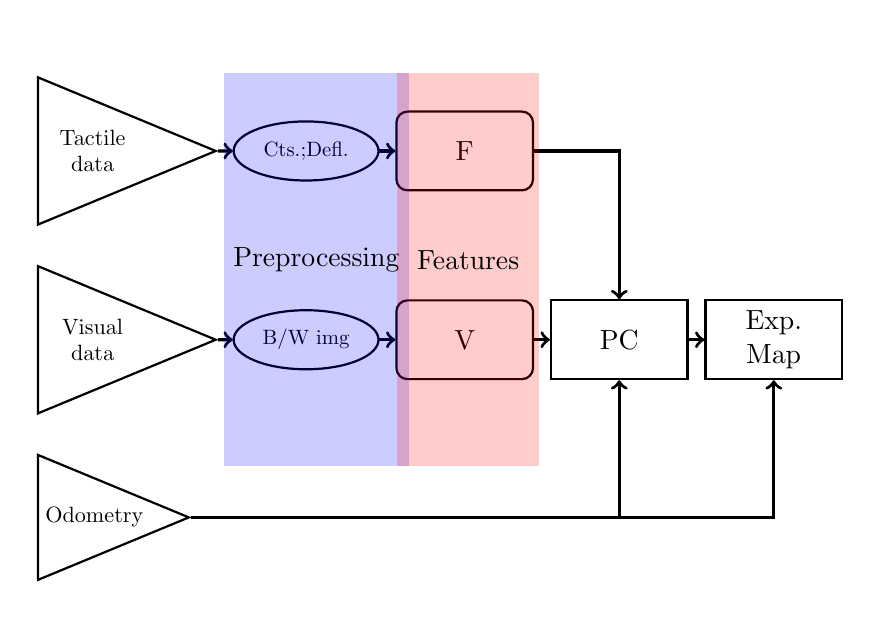
\begin{tikzpicture}[
				round boxes/.style={draw, rectangle,%
                thick,minimum height=1cm, rounded corners,
                minimum width=1cm, black, text=black,
                text width=15mm, anchor=center, align=center},
                boxes/.style={draw, rectangle,%
                thick,minimum height=1cm,
                minimum width=1cm, black, text=black,
                text width=15mm, anchor=center, align=center}, 
    			% Define styles for some special nodes
   				right iso/.style={isosceles triangle,scale=0.8,sharp corners, anchor=center, xshift=-4mm},
    			left iso/.style={right iso, rotate=180, xshift=-8mm},
    			txt/.style={text width=1.5cm,anchor=center},
    			ellip/.style={ellipse,scale=0.75},
    			empty/.style={draw=none}
    			]
  \matrix (mat) [matrix of nodes, nodes=boxes, column sep=0.2cm, row sep=0.5cm] 
  {
                 &   &   &           &           \\ 
    |[right iso]|{Tactile data} & |[ellip]|{Cts.;Defl.} & |[round boxes]|{F} &           &           \\
    |[right iso]|{Visual data} & |[ellip]|{B/W img} & |[round boxes]|{V} & PC & Exp. Map \\
    |[right iso]|{Odometry}     &   &   &           &           \\
  };  
  
%% Node ordering: [row- column]
%% Tactile data
\draw [very thick, black, ->](mat-2-1)--(mat-2-2);
\draw [very thick, black, ->](mat-2-2)--(mat-2-3);
\draw [very thick, black, ->](mat-2-3)-|(mat-3-4);
%%
%%
%%%%% Visual data

\draw [very thick, black, ->](mat-3-1)--(mat-3-2);
\draw [very thick, black, ->](mat-3-2)--(mat-3-3);
\draw [very thick, black, ->](mat-3-3)--(mat-3-4);
\draw [very thick, black, ->](mat-3-4)--(mat-3-5);


%%
%%%% Odometry info connections
\draw [very thick, black, ->](mat-4-1)-|(mat-3-4);
\draw [very thick, black, ->](mat-4-1)-|(mat-3-5);


%%
%%%% Obj Map and Exp Map fusion to Vita Map
%\draw [very thick, black, ->](mat-3-5)-|(mat-4-6);
%\draw [very thick, black, ->](mat-5-5)-|(mat-4-6);

%% Bounding rectangles
% draw the rectangles
\node at(-2.75cm, .5cm) [right,fill=blue,text opacity=1,opacity=.2, minimum width=1.8cm, minimum height=5cm, text height=-4.cm] {Preprocessing};

\node at(-0.55cm, .5cm) [right,fill=red,text opacity=1,opacity=.2, minimum width=1.8cm, minimum height=5cm, text height=-4.2cm] {Features};


\end{tikzpicture}
\end{document}